\documentclass[11pt]{article}

\usepackage[a4paper,margin=1in]{geometry}
\usepackage{amsmath,amssymb,amsthm}
\usepackage{booktabs}
\usepackage{graphicx}
\usepackage{hyperref}
\usepackage{array}
\usepackage{caption}
\usepackage{enumitem}

\graphicspath{{../figures/}{figures/}}

\title{A Three-Layer Empirical Residual Law for Consecutive Prime Gaps:\\ Drift and Modular Resonance}
\author{Jose A. Cano Gregorio}
\date{Version 0.3 draft}

\newtheorem{conjecture}{Conjecture}

\begin{document}
\maketitle

\noindent\textbf{Status:} empirical white paper / structural conjecture \\
\textbf{Primary model family:} \texttt{V44\_PRIMES\_PREDICTOR\_FROZEN} \\
\textbf{Primary experimental baseline:} \texttt{V15\_CAUSAL}, \texttt{resid\_log} \\
\textbf{Primary validation blocks:} B07--B10 \\
\textbf{Date:} 2026-05-07

\vspace{1em}
\hrule
\vspace{1em}

\begin{abstract}
We study the residual structure of consecutive prime-gap pairs after a causal sieve-inspired baseline model. For consecutive prime gaps
\[
g_1=p_{n+1}-p_n,\qquad g_2=p_{n+2}-p_{n+1},
\]
we introduce the variables
\[
S=g_1+g_2,\qquad D=g_2-g_1,\qquad t=\log\log p_n.
\]
Empirically, the logarithmic residual admits a three-layer decomposition consisting of a static geometric envelope in \(S\), a smooth scale-dependent drift in \(S\) and \(D^2\), and an even modular resonance with wavelength \(\Lambda=45\) in the \(S,D\) coordinate representation. The resonant term survives rolling causal validation, geometric null controls, comparison against smooth polynomial alternatives, and comparison against a more flexible two-dimensional Fourier form.

We present the resulting law as an empirical structural conjecture:
\[
\Delta(S,D;p)=E_0(S)+U(S,D;\log\log p)+R_{45}(S,D;\log\log p)+\mathcal{E}(S,D;p).
\]
The present work does not prove the Riemann Hypothesis, the twin prime conjecture, Goldbach's conjecture, or any asymptotic theorem. Its contribution is to isolate a reproducible, non-random signal in the local distribution of primes.
\end{abstract}

\section{Introduction}

The distribution of prime numbers is commonly modeled through global asymptotic laws, local congruence constraints, and Hardy--Littlewood-type heuristics. Yet even after a strong sieve-inspired baseline is applied, local residuals in the geometry of consecutive gaps exhibit persistent patterns.

In this paper, we document the discovery of a three-layer residual law. This law suggests that the error in predicting consecutive gaps is not featureless noise but contains a systematic drift and a modular resonance anchored to a specific geometric wavelength \((\Lambda=45)\).

After a baseline model is removed, the remaining logarithmic residual is well described by three components:
\begin{enumerate}[label=\arabic*.]
\item a static envelope depending primarily on \(S=g_1+g_2\);
\item a smooth scale-dependent drift in \(S\) and \(D^2\);
\item a modular resonant term, even in \(D=g_2-g_1\), with wavelength \(\Lambda=45\).
\end{enumerate}

The main empirical law is
\[
\Delta(S,D;p)=E_0(S)+U(S,D;t)+R_{45}(S,D;t)+\mathcal{E}(S,D;p),\qquad t=\log\log p.
\]

The term \(R_{45}\) is the central finding: after removal of the smooth drift, a resonance with separable geometry in \(S\) and \(D\) remains. The resonance is not materially improved by a more flexible Full2D Fourier form and is not reproduced by geometric null controls.

\section{Definitions}

Let \(p_n\) denote the \(n\)-th prime. Define consecutive gaps
\[
g_1=p_{n+1}-p_n,\qquad g_2=p_{n+2}-p_{n+1}.
\]
We use the coordinates
\[
S=g_1+g_2,\qquad D=g_2-g_1.
\]
It is also useful to introduce semi-gaps
\[
A=\frac{g_1}{2},\qquad B=\frac{g_2}{2}.
\]
Then
\[
A+B=\frac{S}{2},\qquad B-A=\frac{D}{2}.
\]

The scale variable used in the parametric version of the law is
\[
t=\log\log p,
\]
where \(p\) denotes the representative prime scale of the block, typically \(p_n\) or a block center.

Let \(H(S,D;p)\) denote the observed empirical mass for gap-pair geometry in a block near scale \(p\). Let \(W_0(S,D;p)\) denote a causal baseline weight produced by the selected sieve-inspired model. The primary logarithmic residual is
\[
\Delta(S,D;p)=\log\frac{H(S,D;p)}{W_0(S,D;p)}
\]
or the corresponding stabilized logarithmic residual used in the computation.

In the experiments reported here, the primary baseline is the \texttt{V15\_CAUSAL} residual model and the primary target is \texttt{resid\_log}.

\section{Baseline and experimental protocol}

The experiments are conducted in a rolling causal setting. Blocks are ordered by increasing prime scale. A model component evaluated on a test block may only use information from earlier blocks.

This constraint is essential. Many candidate structures fit well in-sample but fail when parameters are extrapolated causally. The reported law survived the following classes of tests:
\begin{itemize}
\item rolling causal validation;
\item comparison to an envelope-only model;
\item comparison to a smooth drift model;
\item comparison to higher-order smooth alternatives;
\item comparison to a more flexible two-dimensional Fourier model;
\item geometric null controls based on shuffling \(D\);
\item wavelength sweeps for the resonant term.
\end{itemize}

The primary metrics are RMS reduction and median improvement percentage relative to the specified baseline residual. When a component is reported as improving another component, the improvement is measured after the previous component has already been removed.

\section{The three-layer residual law}

The empirical law decomposes the residual into
\[
\Delta(S,D;p)=E_0(S)+U(S,D;t)+R_{45}(S,D;t)+\mathcal{E}(S,D;p).
\]

\subsection{Static envelope}

The static envelope is modeled as
\[
E_0(S)=c_0+c_1\sqrt S+c_2\log(1+S)+c_3S^{-1/2}.
\]
This term captures the dominant static dependence of the residual on the total two-gap span \(S\).

\subsection{Smooth scale-dependent drift}

After removing \(E_0\), a smooth deformation remains. Empirically, the following form captures it:
\[
U(S,D;t)=u_0(t)+u_1(t)(S-\bar S_t)+u_2(t)(D^2-\overline{D^2}_t).
\]

Here \(\bar S_t\) and \(\overline{D^2}_t\) are centering conventions. In production-style prediction, they must be computed without observing future targets. Two valid choices are:
\begin{enumerate}[label=\arabic*.]
\item support-based centers, computed from the candidate grid being scored;
\item fixed reference centers, learned once from the training support.
\end{enumerate}

The function \(u_2(t)\) is empirically small and comparatively stable, while \(u_0(t)\) and \(u_1(t)\) are strongly predictable functions of \(t=\log\log p\) in the tested range.

\subsection{Modular resonance}

After removing the smooth drift, a resonant component remains:
\[
R_{45}(S,D;t)
=
\cos\left(\frac{\pi D}{45}\right)
\left[
a(t)\sin\left(\frac{\pi S}{45}\right)
+
b(t)\cos\left(\frac{\pi S}{45}\right)
\right].
\]

This term is even in \(D\), separable in \(S\) and \(D\), and has wavelength \(\Lambda=45\) in the \(S,D\) coordinate representation.

\section{Trigonometric origin of the separable form}

The separable \(S,D\) form is not arbitrary. It arises naturally from symmetric oscillations in the semi-gap coordinates \(A\) and \(B\).

Consider
\[
\sin\left(\frac{2\pi A}{T}\right)+\sin\left(\frac{2\pi B}{T}\right).
\]
Using
\[
\sin x+\sin y=2\sin\left(\frac{x+y}{2}\right)\cos\left(\frac{x-y}{2}\right),
\]
we obtain
\[
\sin\left(\frac{2\pi A}{T}\right)
+
\sin\left(\frac{2\pi B}{T}\right)
=
2\sin\left(\frac{\pi S}{2T}\right)
\cos\left(\frac{\pi D}{2T}\right).
\]
Thus a symmetric oscillation in the two semi-gaps becomes a product that is even in \(D\) in the \(S,D\) coordinates.

The empirically observed resonant term is written directly as
\[
R_{45}(S,D;t)
=
\cos\left(\frac{\pi D}{45}\right)
\left[
a(t)\sin\left(\frac{\pi S}{45}\right)
+
b(t)\cos\left(\frac{\pi S}{45}\right)
\right].
\]

This structure was compared against a more flexible Full2D form containing both even and odd terms in \(D\). The Full2D form did not materially improve performance, supporting the separable structure that is even in \(D\).

\section{Causal validation}

The following table summarizes the primary V44b audit. Improvements are reported as percentage RMS reductions in a rolling causal setup.

\begin{table}[htbp]
\centering
\begin{tabular}{rrrrrr}
\toprule
Block & \(M3\) vs \(M0\) & \(R45\) vs \(M3\) & Smooth vs \(M3\) & Full2D vs \(M3\) & Null vs \(M3\)\\
\midrule
B07 & +26.87\% & +8.19\% & +0.16\% & +8.18\% & -11.07\%\\
B08 & +32.37\% & +3.94\% & +0.09\% & +3.94\% & -8.25\%\\
B09 & +38.17\% & +2.06\% & +0.17\% & +1.97\% & -2.77\%\\
B10 & +38.71\% & +1.11\% & +0.20\% & +1.11\% & -0.34\%\\
\bottomrule
\end{tabular}
\caption{Primary causal validation table. Improvements are percentage RMS reductions.}
\label{tab:v44b}
\end{table}

The results support four empirical conclusions. First, the smooth drift \(M3=E_0+U\) is the dominant correction beyond the baseline. Second, \(R_{45}\) provides an additional positive causal correction in all tested blocks. Third, a smooth incremental extension using higher-order terms such as \(S^2\) and \(SD^2\) contributes only weakly. Fourth, a more flexible Full2D resonant model does not materially improve upon the separable \(R_{45}\), while a \(D\)-shuffle null destroys the resonant improvement.

\begin{figure}[htbp]
\centering
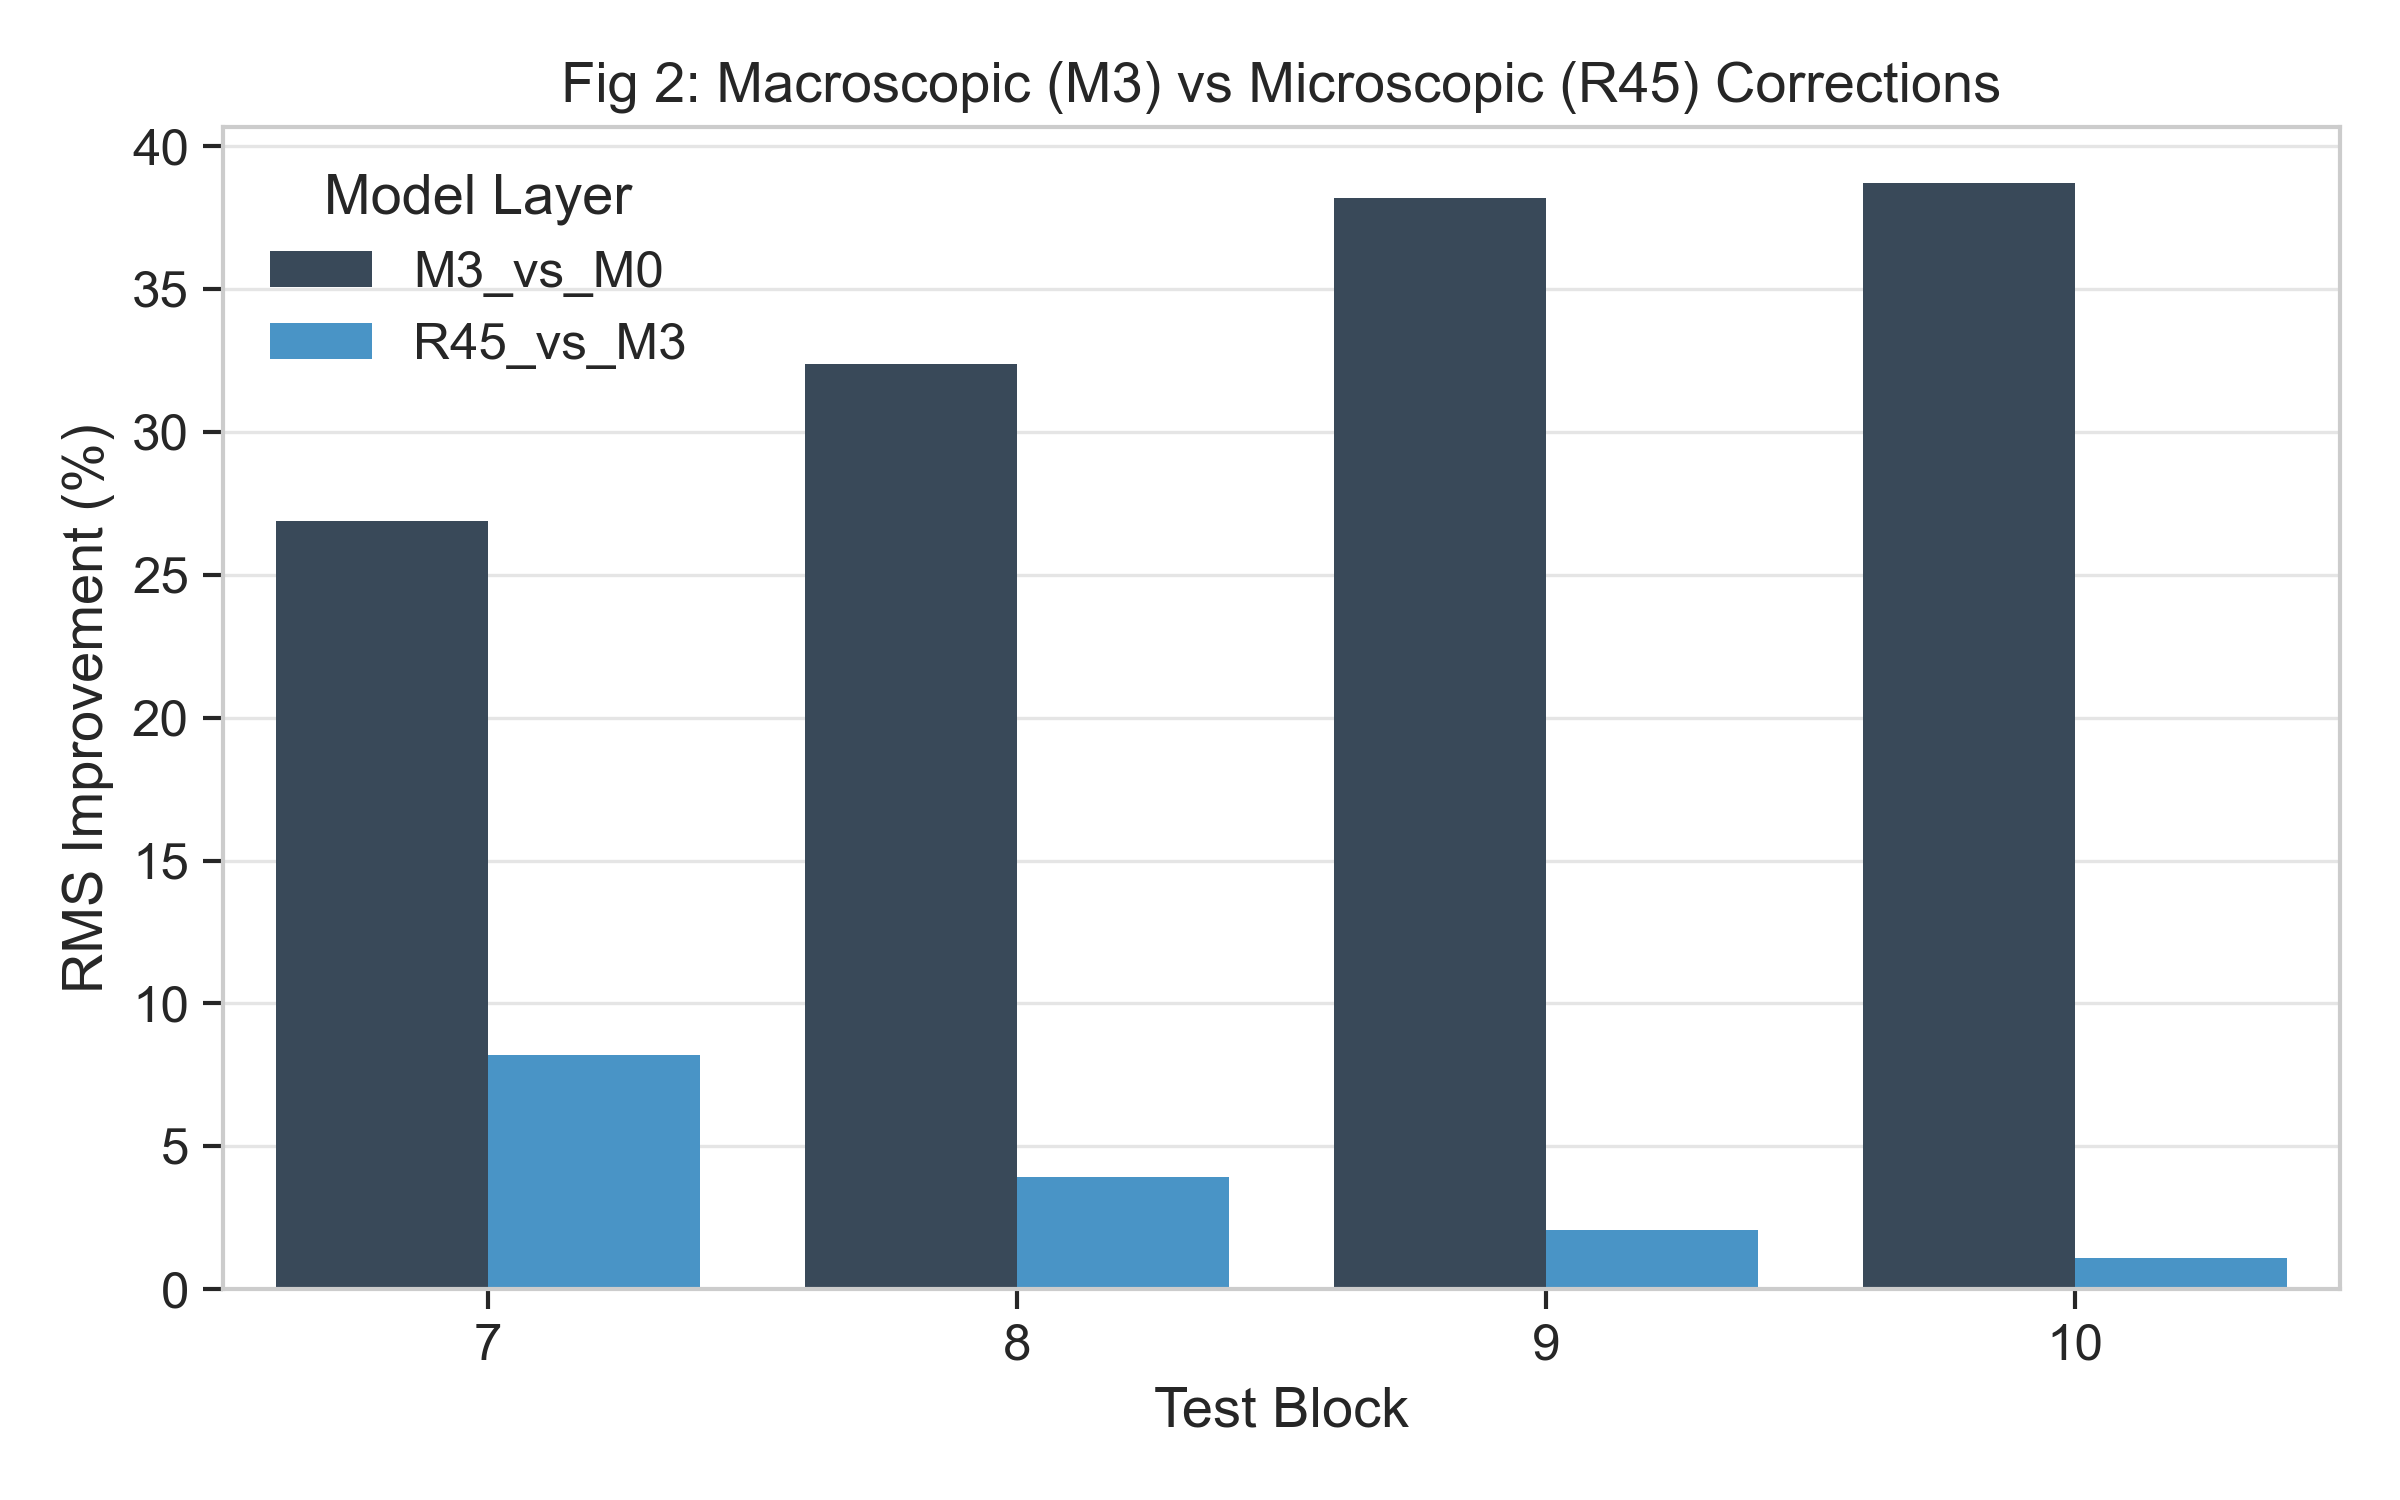
\includegraphics[width=0.95\linewidth]{fig2_v44b_overview.png}
\caption{Causal validation overview. The smooth drift \(M3\) provides the dominant macroscopic correction over \(M0\), while \(R45\) adds a smaller but consistently positive residual correction on top of \(M3\).}
\label{fig:v44b-overview}
\end{figure}

\section{Wavelength sweep and the \texorpdfstring{\(\Lambda=45\)}{Lambda=45} peak}

After removing the smooth drift, the resonant wavelength was scanned over a range of \(\Lambda\). The median causal improvement showed a local maximum around \(\Lambda=45\).

Representative median improvements:
\begin{table}[htbp]
\centering
\begin{tabular}{rr}
\toprule
\(\Lambda\) & Median causal improvement\\
\midrule
30 & +1.82\%\\
35 & +3.26\%\\
40 & +3.94\%\\
44 & +4.18\%\\
45 & +4.19\%\\
46 & +4.17\%\\
50 & +3.86\%\\
60 & +2.45\%\\
90 & +0.65\%\\
\bottomrule
\end{tabular}
\caption{Representative wavelength sweep after removing the smooth drift.}
\label{tab:lambda-sweep}
\end{table}

The improvement is not a single isolated point. It forms a smooth peak around \(44\leq\Lambda\leq46\), with \(\Lambda=45\) as the median maximum in the tested regime.

The final tested block showed weaker signal and a local displacement toward smaller wavelengths. This may indicate a finite-range regime change, a low signal-to-noise effect, or phase/amplitude drift. We do not interpret it as conclusive evidence of a chirp.

\begin{figure}[htbp]
\centering
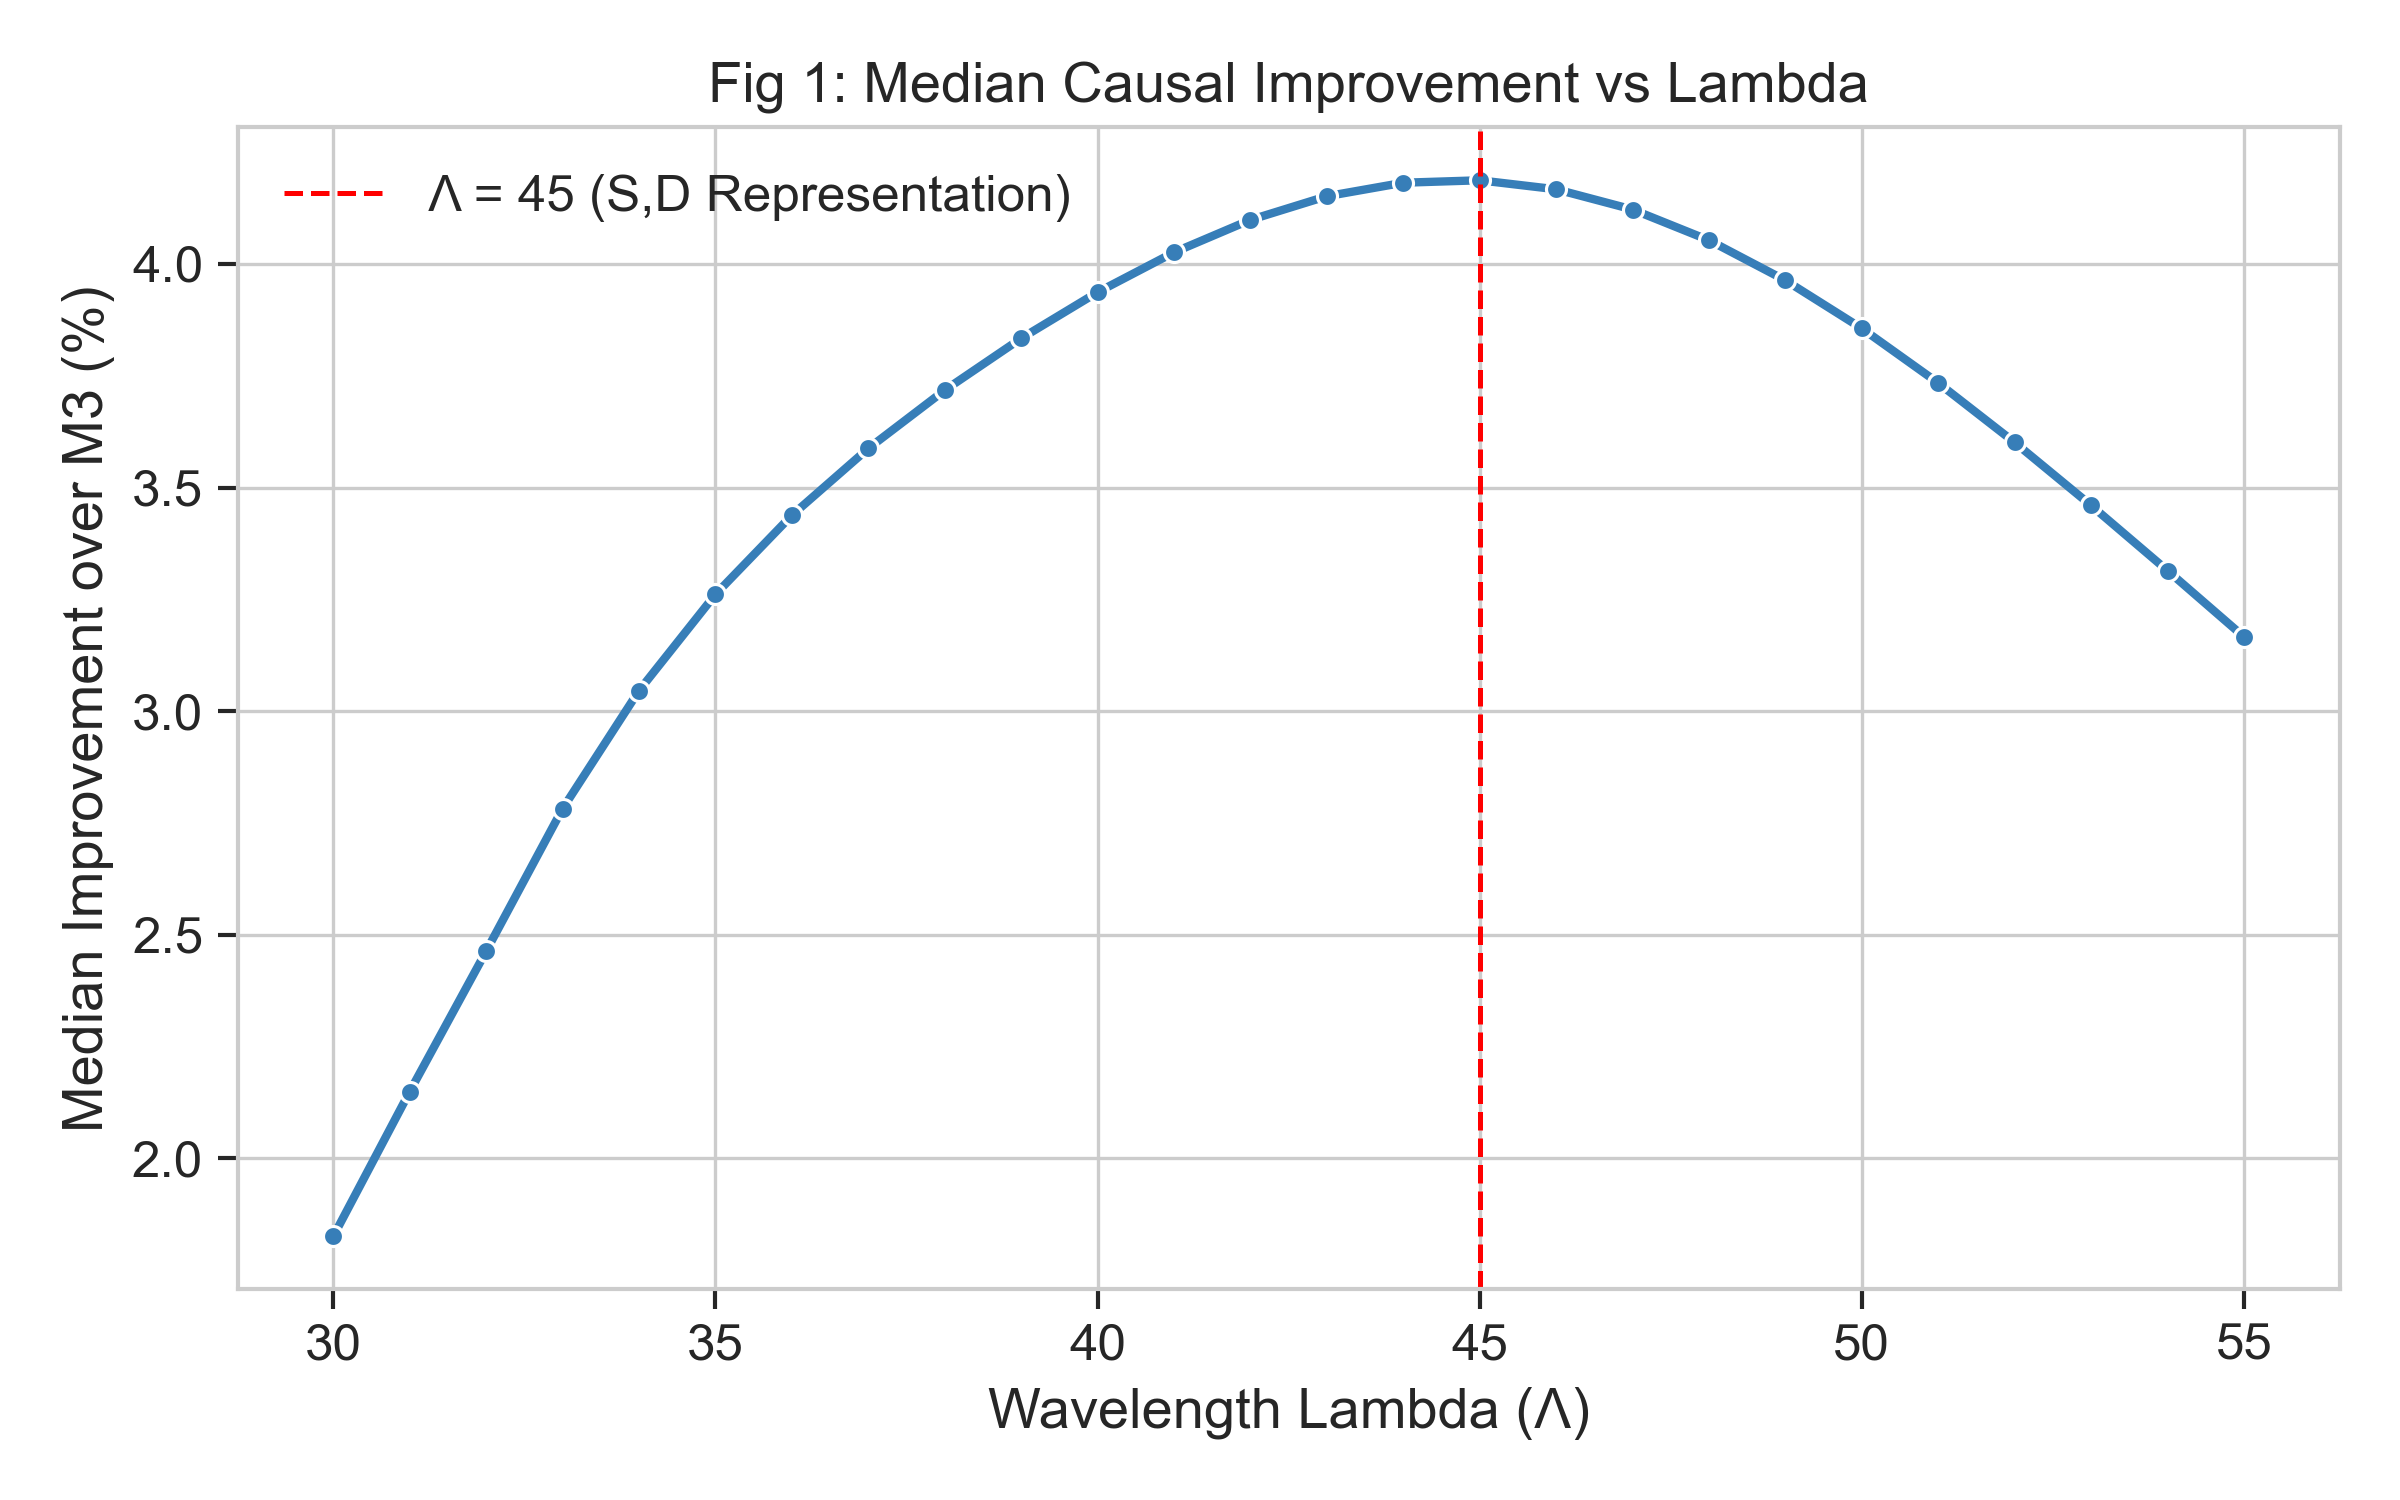
\includegraphics[width=0.95\linewidth]{fig1_lambda_sweep.png}
\caption{Wavelength sweep after removal of the smooth drift. The median causal improvement peaks at \(\Lambda=45\), with nearby values \(\Lambda=44\) and \(\Lambda=46\) nearly tied.}
\label{fig:lambda-sweep}
\end{figure}

\section{Null controls and model comparison}

Several falsifiers were used to test whether the resonant term was merely an artifact of interpolation.

\subsection{\texorpdfstring{\(D\)}{D}-shuffle}

The \(D\)-shuffle control disrupts the relationship between the sum coordinate \(S\) and the asymmetry coordinate \(D\). In the primary audit, this control produced negative improvement, indicating that the resonant term depends on the true geometry of the gap pair.

\begin{figure}[htbp]
\centering
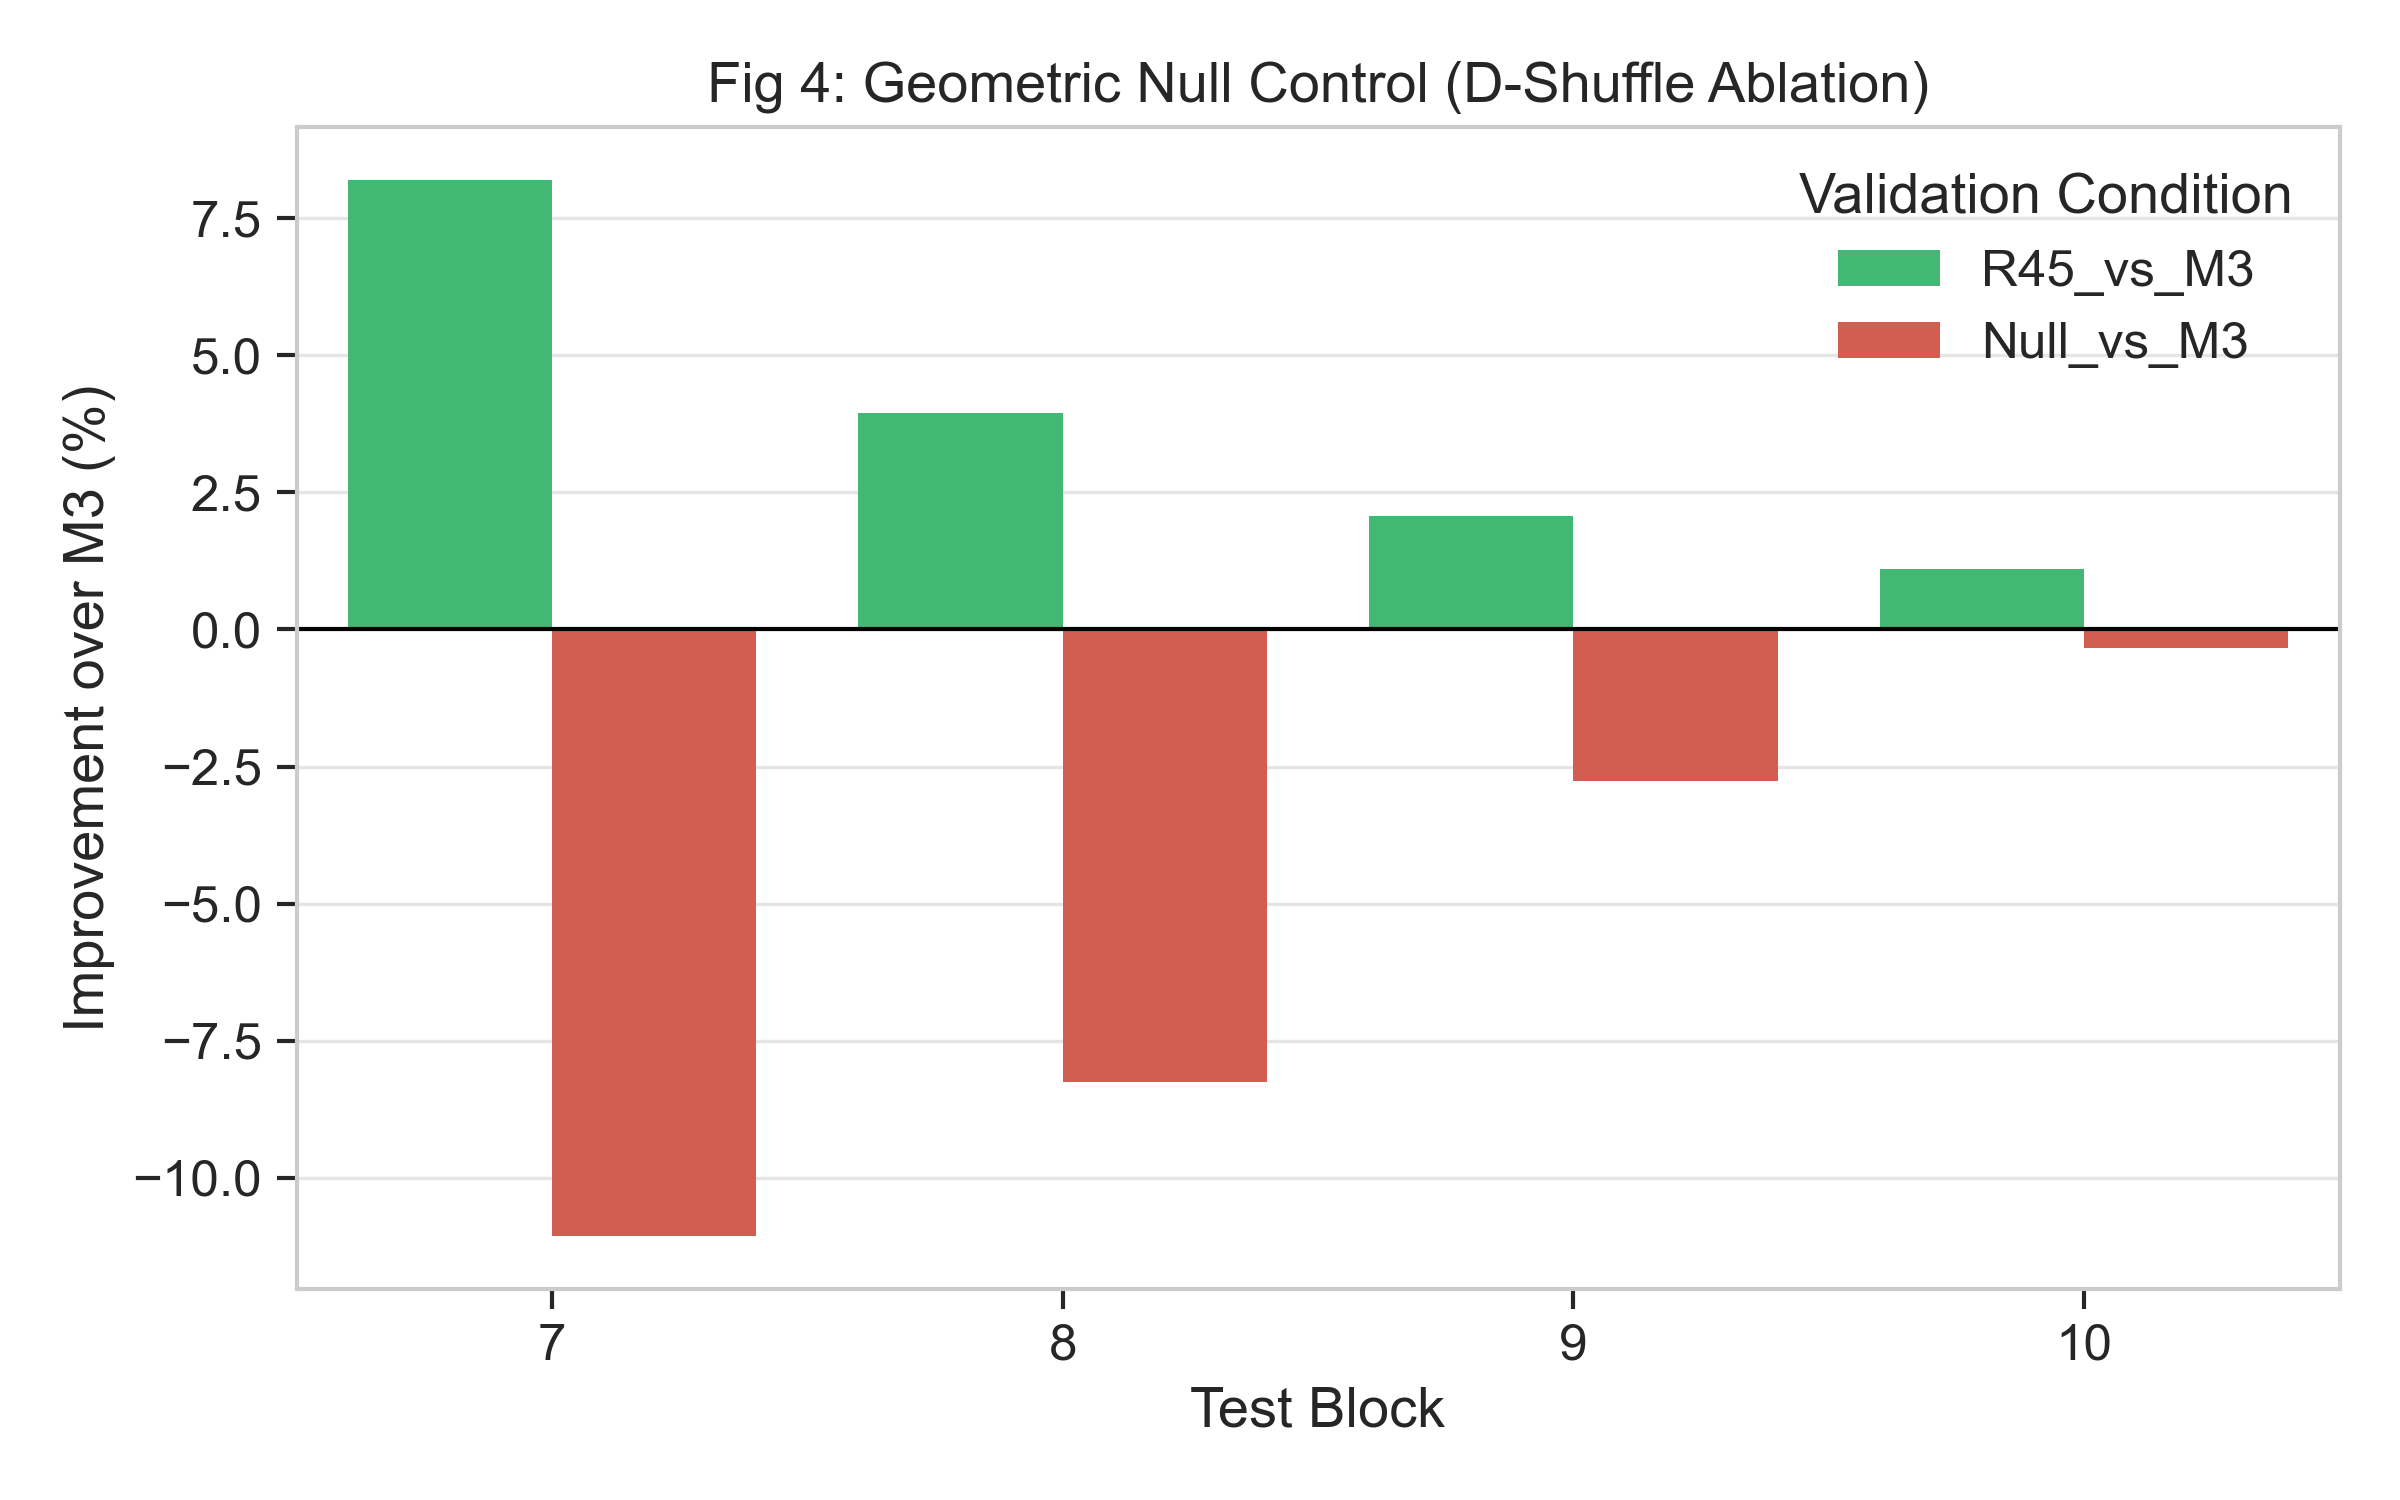
\includegraphics[width=0.95\linewidth]{fig4_null_control.png}
\caption{Geometric null control. The \(D\)-shuffle destroys the improvement associated with the \(R45\) term, indicating that the resonant correction depends on the real coupling between \(S\) and \(D\).}
\label{fig:null-control}
\end{figure}

\subsection{Full2D comparison}

The separable resonance was compared to a more flexible model of the form
\[
\begin{aligned}
&c_1(t)\sin\left(\frac{\pi S}{45}\right)\cos\left(\frac{\pi D}{45}\right)
+c_2(t)\cos\left(\frac{\pi S}{45}\right)\cos\left(\frac{\pi D}{45}\right)\\
&\quad +c_3(t)\sin\left(\frac{\pi S}{45}\right)\sin\left(\frac{\pi D}{45}\right)
+c_4(t)\cos\left(\frac{\pi S}{45}\right)\sin\left(\frac{\pi D}{45}\right).
\end{aligned}
\]

The additional odd-in-\(D\) terms did not materially improve predictive performance. This supports the separable structure that is even in \(D\).

\subsection{Smooth alternatives}

A smooth incremental alternative using additional polynomial-like features was also tested. Such terms contributed only weakly relative to \(R_{45}\). This suggests that the resonant term is not merely a disguised smooth drift term.

\begin{figure}[htbp]
\centering
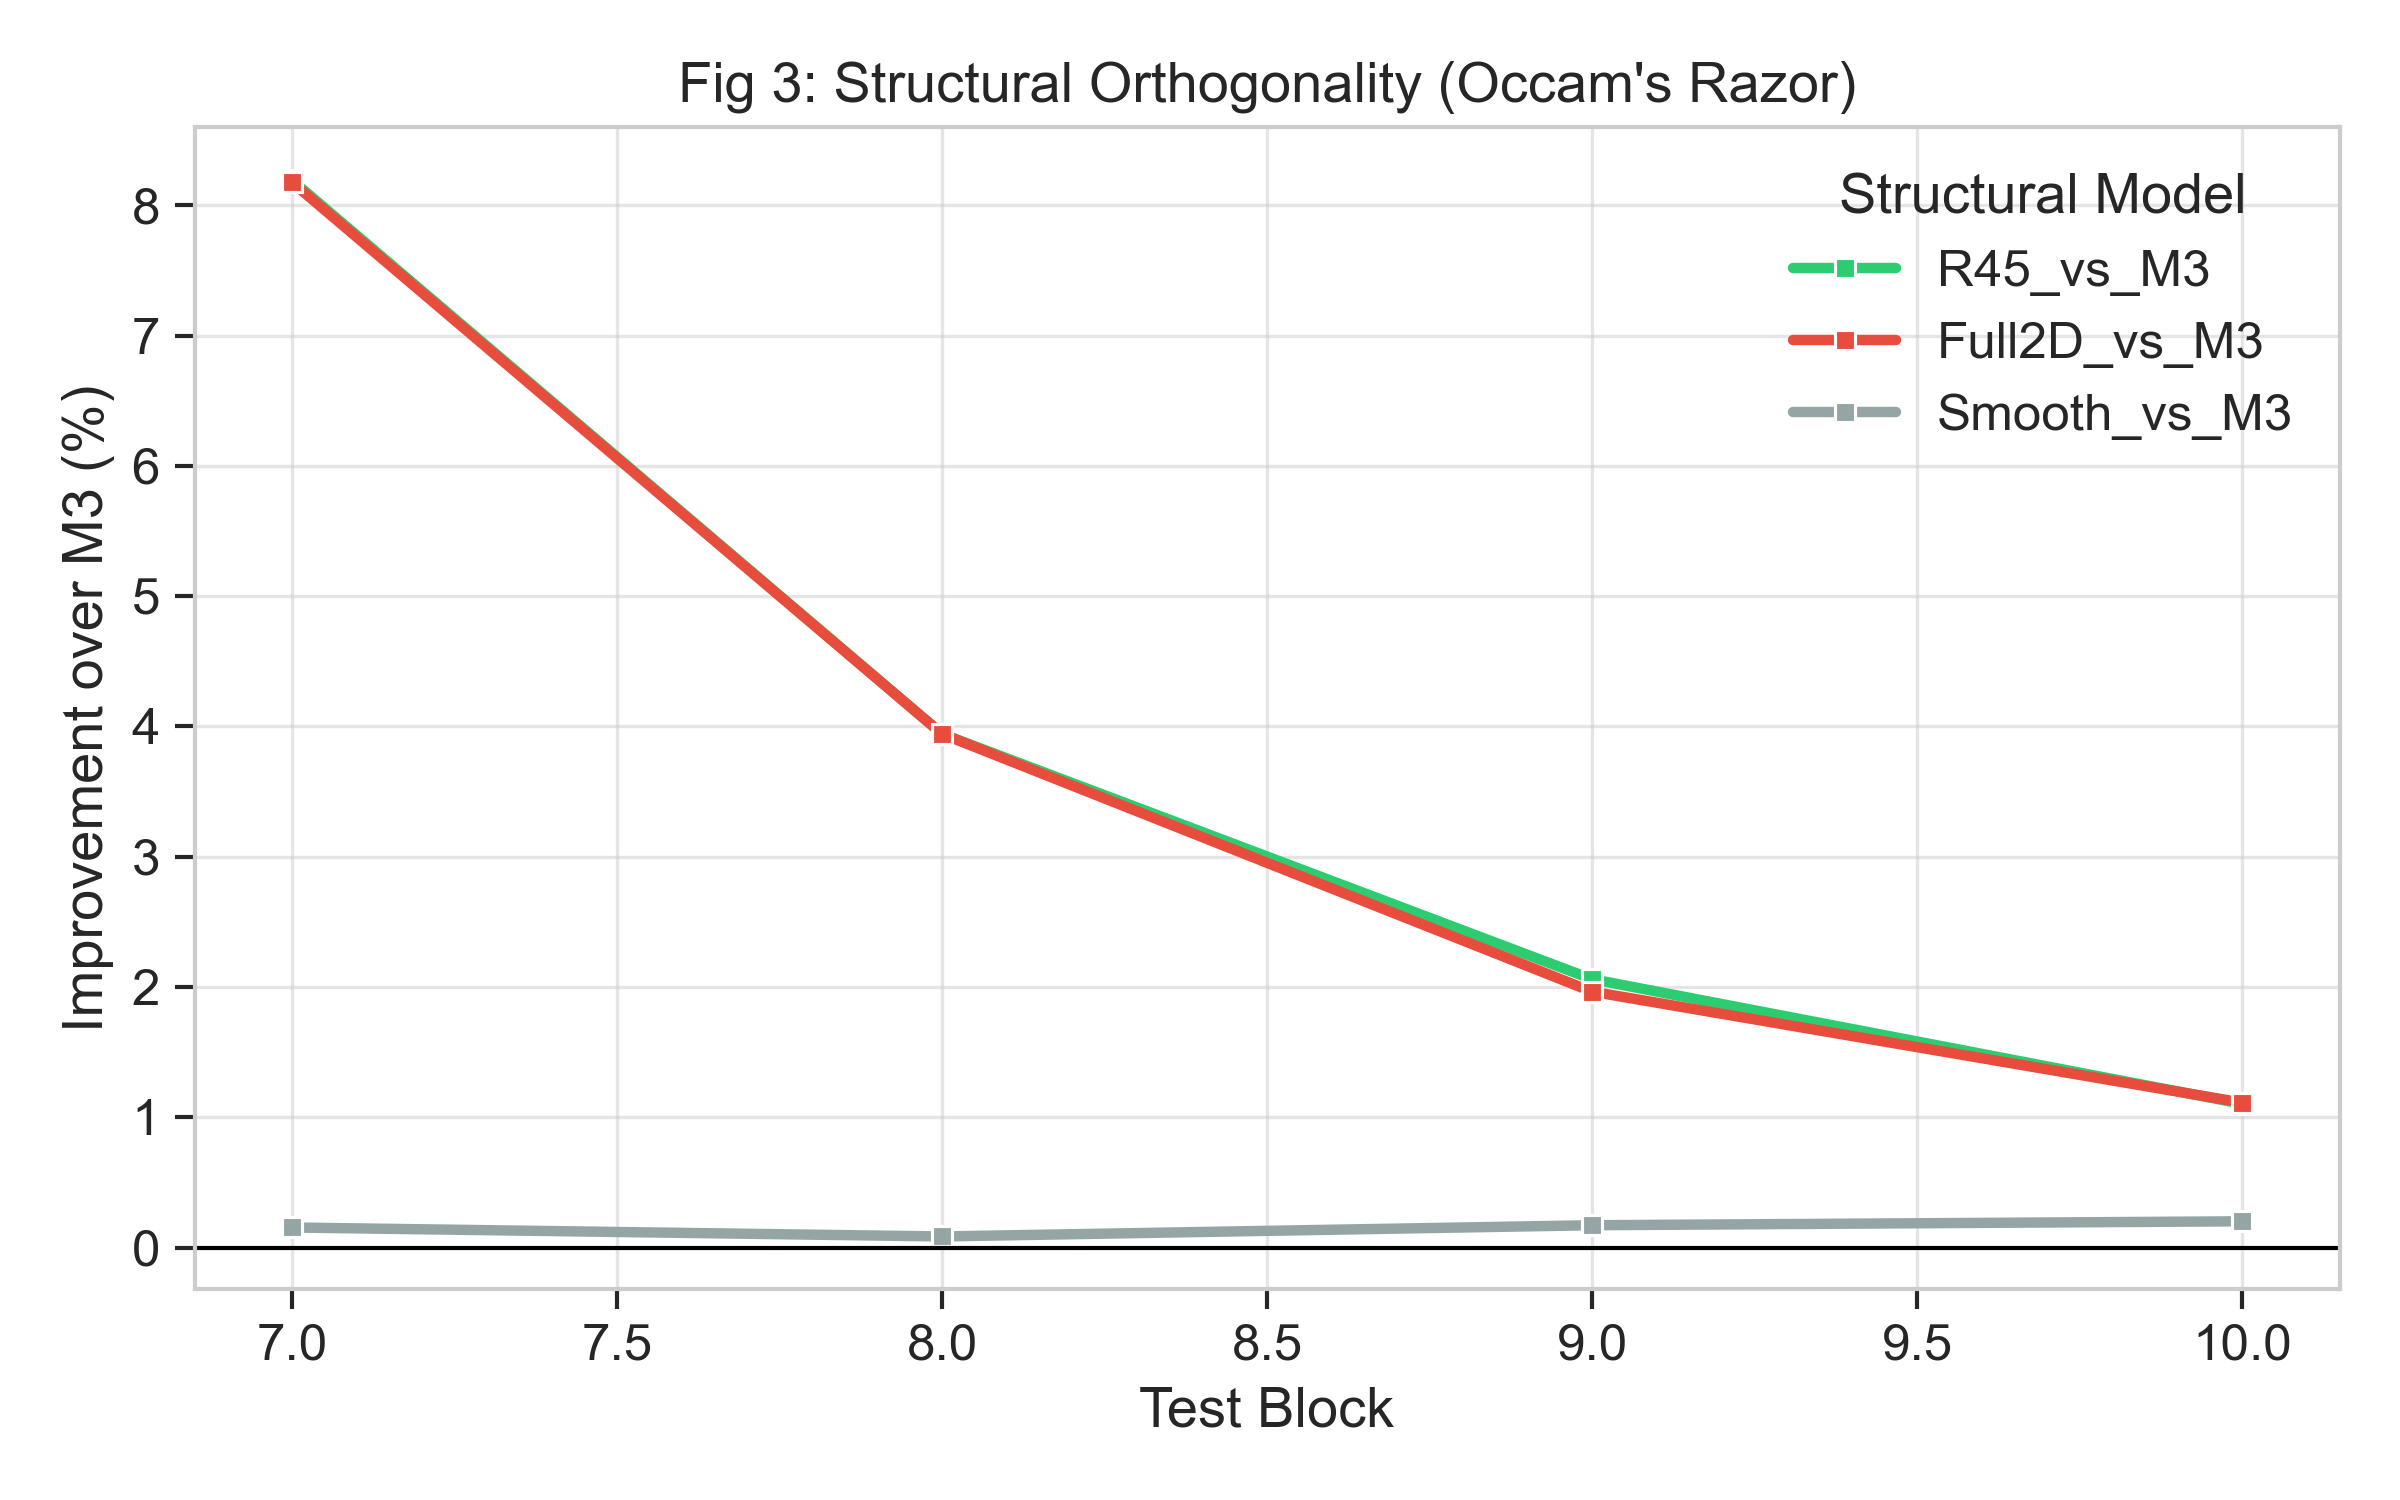
\includegraphics[width=0.95\linewidth]{fig3_model_ablation.png}
\caption{Model ablation. The separable \(R45\) term tracks the more flexible Full2D model, while SmoothNested contributes only weakly after \(M3\).}
\label{fig:model-ablation}
\end{figure}

\section{Parameter evolution}

The predictor uses scale-dependent coefficients, with \(t=\log\log p\). The smooth drift parameters \(u_0(t)\) and \(u_1(t)\), and the resonant coefficients \(a(t)\) and \(b(t)\), are estimated causally from earlier blocks.

The coefficient \(b(t)\) is constrained by a cooling rule: it remains non-positive and is not allowed to become more negative than the last causally observed value without validation. This prevents over-excitation of the resonant term in high blocks.

\begin{figure}[htbp]
\centering
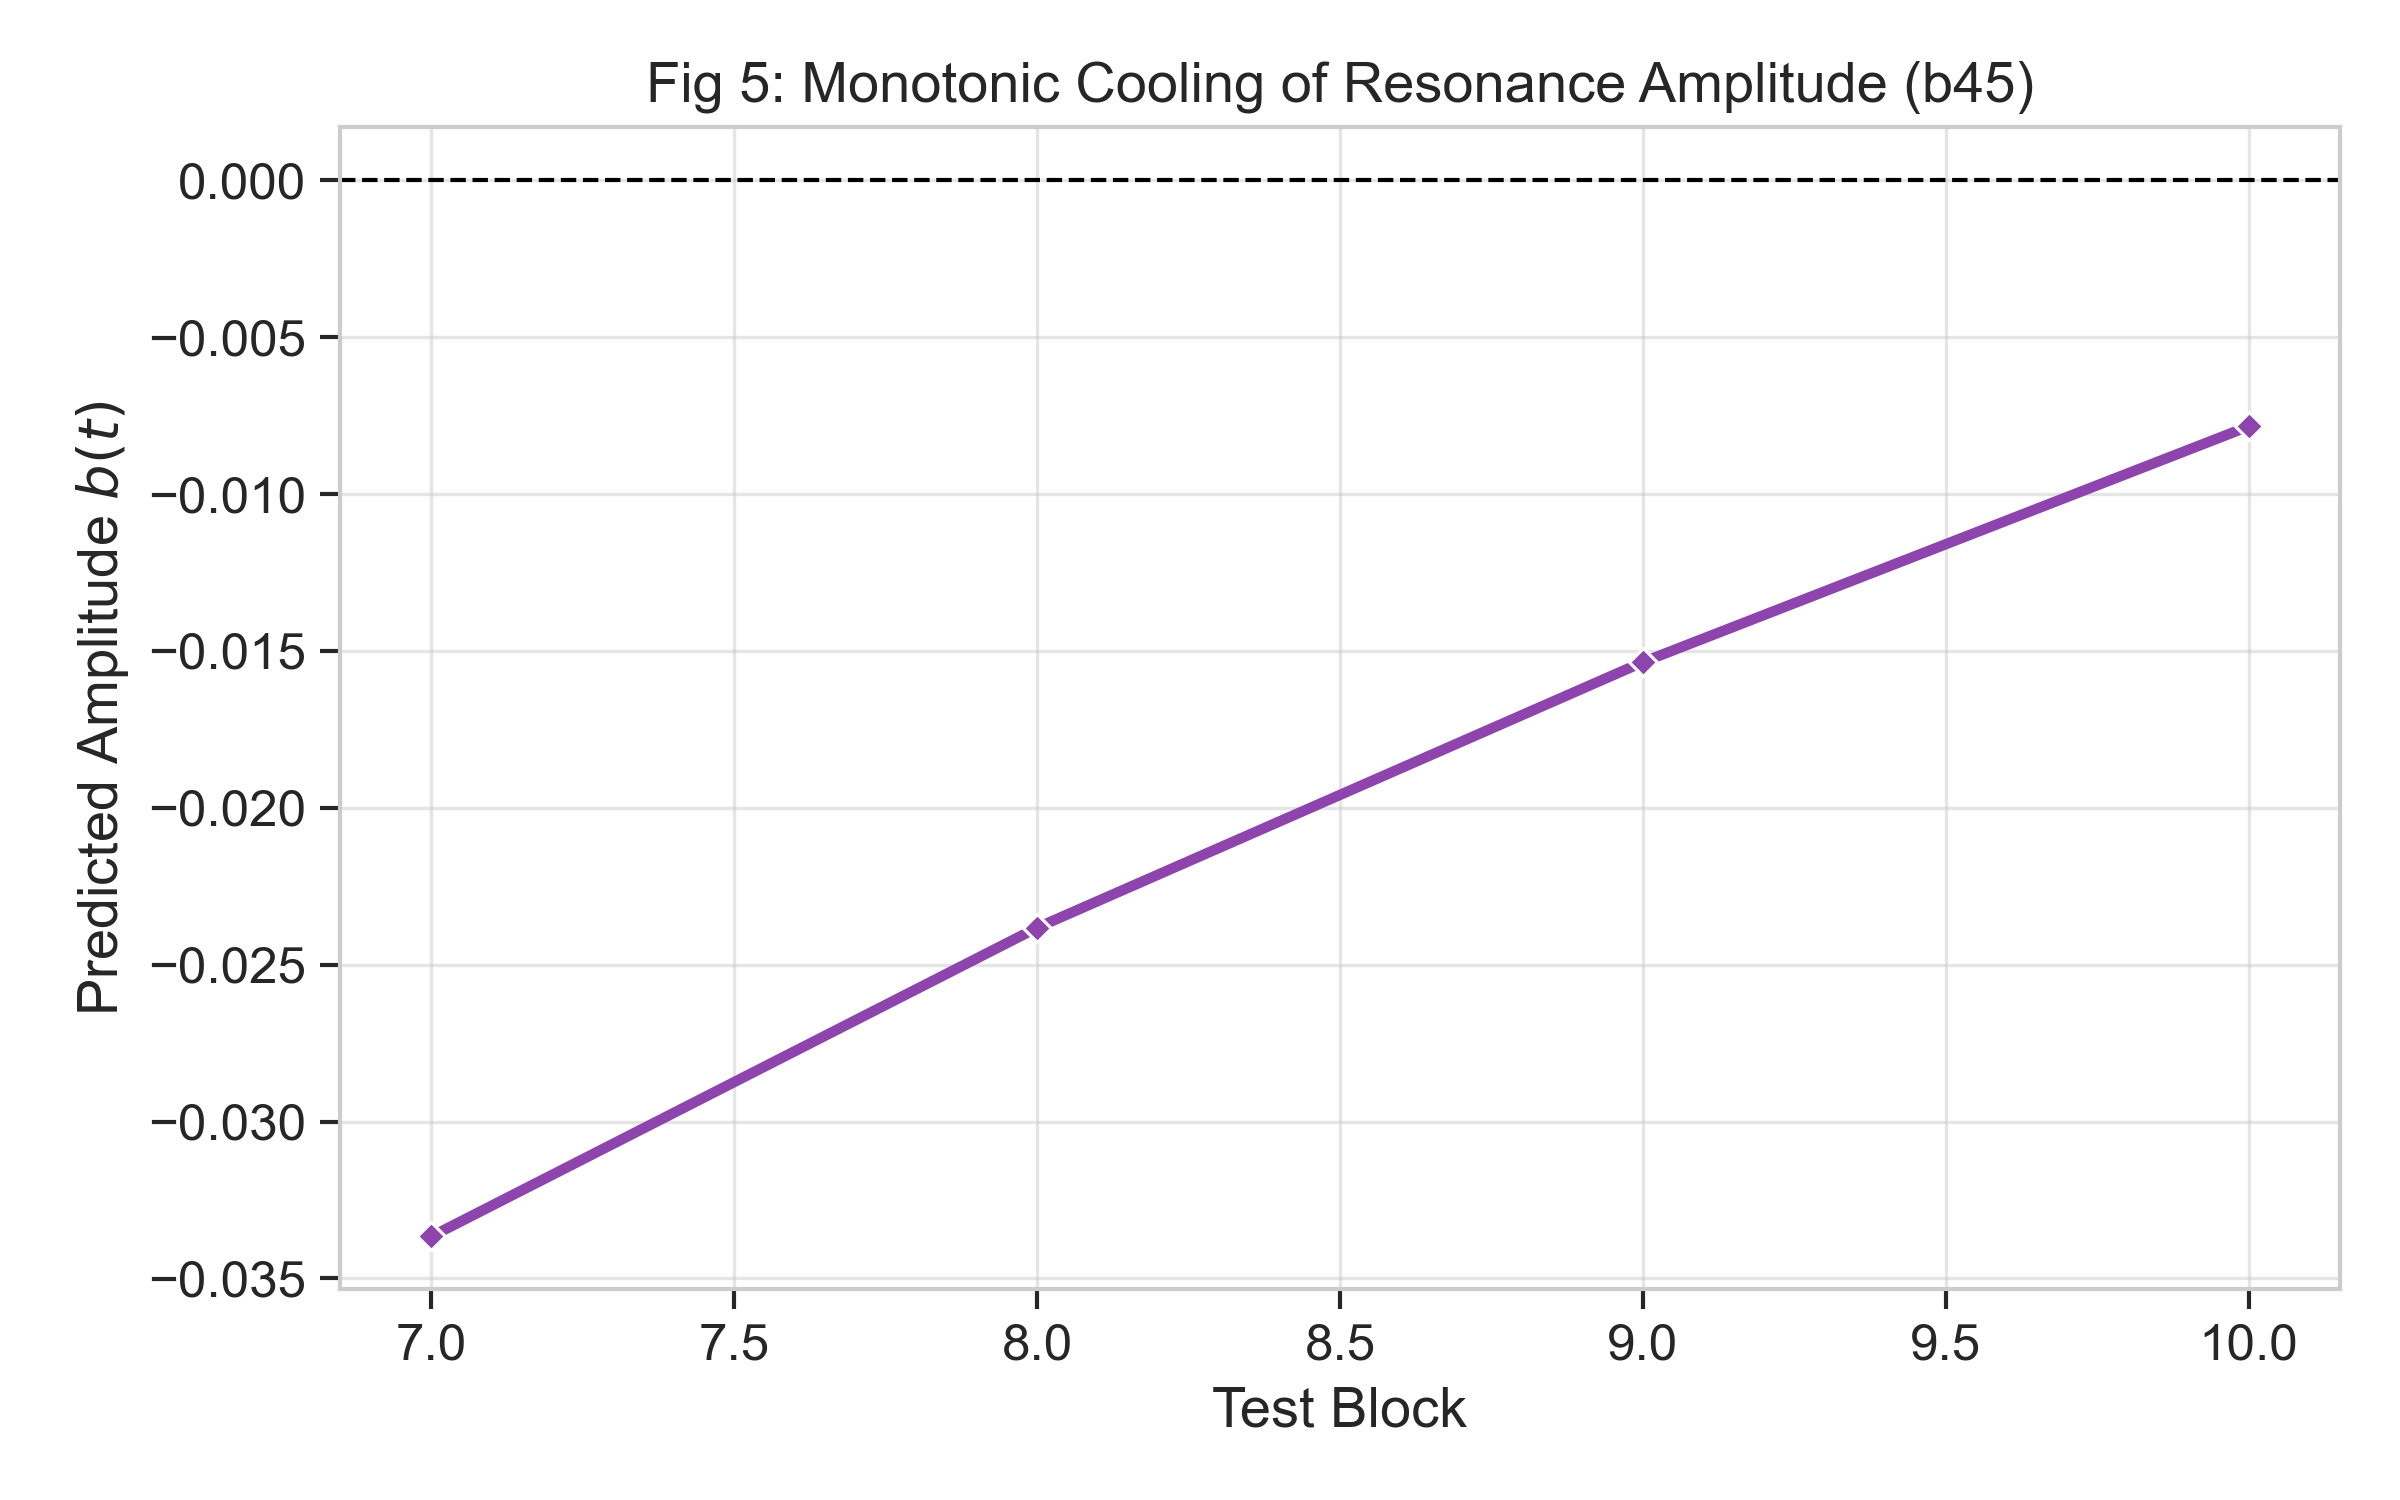
\includegraphics[width=0.95\linewidth]{fig5_parameter_evolution.png}
\caption{Parameter evolution. The resonant coefficient \(b_{45}\) cools toward zero, while the remaining coefficients evolve smoothly over the tested blocks.}
\label{fig:parameter-evolution}
\end{figure}

\section{Empirical structural conjecture}

The experiments motivate the following structural conjecture.

\begin{conjecture}
For consecutive prime-gap pairs over bounded gap ranges and with respect to an appropriate causal sieve baseline \(W_0\), the structured component of the logarithmic residual admits a decomposition
\[
\Delta(S,D;p)=E_0(S)+U(S,D;\log\log p)+R_{45}(S,D;\log\log p)+\mathcal{E}(S,D;p),
\]
where \(E_0\) is a static envelope in \(S\), \(U\) is a smooth scale-dependent drift in \(S\) and \(D^2\), and \(R_{45}\) is the dominant modular resonant component after removal of the smooth drift. The remaining error \(\mathcal{E}\) is empirically smaller and less structured under the tested regimes.
\end{conjecture}

This is an empirical conjecture. No asymptotic bound is proved here for \(\mathcal{E}\).

\section{Limitations}

The present work has several important limitations.
\begin{enumerate}[label=\arabic*.]
\item The validation is finite-range and computational.
\item The primary reported validation is based on the \texttt{V15\_CAUSAL} logarithmic residual \texttt{resid\_log}.
\item The law has not yet been converted into an analytic error bound.
\item The result does not prove the Riemann Hypothesis, the twin prime conjecture, Goldbach's conjecture, or any other open asymptotic theorem.
\item The behavior of the residual under larger prime ranges and alternative baselines remains to be studied.
\item The centering conventions \(\bar S_t\) and \(\overline{D^2}_t\) must be handled carefully in production-style prediction to avoid future leakage.
\end{enumerate}

These limitations are not peripheral. They mark the difference between an empirical structural law and a mathematical theorem.

\section{Future work}

The immediate next step is to validate the three-layer law on larger and independent ranges.

Three future directions are especially natural.

\subsection{Fixed-gap marginalization}

The formula may be projected onto fixed-gap statistics by summing over one gap coordinate. In particular, one may study whether the corrected mass for \(g_1=2\) yields a refined empirical heuristic for twin-gap statistics.

\subsection{Global error accumulation}

The local residual law may be accumulated over prime ranges to study whether the residual error after subtracting \(E_0+U+R_{45}\) exhibits a reduced global growth rate.

\subsection{Analytic sieve interpretation}

A long-term goal is to interpret the three-layer law in terms of explicit sieve weights or corrections to Hardy--Littlewood-type heuristics. The main mathematical challenge is to derive a rigorous error term.

\section{Reproducibility}

The companion repository contains a frozen implementation of the V44 predictor and minimal scripts for reproducing the primary validation tables and figures.

The central implementation exposes the following API:
\begin{verbatim}
predict_delta(p_center, g1, g2)
predict_weight_correction(p_center, g1, g2)
score_gap_pair(p_center, g1, g2)
audit_dataframe(df)
\end{verbatim}

The repository is intentionally scoped to consecutive gap-pair residuals. Applications to fixed-gap marginalization and global error accumulation are left for future work.

\section{Disclosure of AI assistance}

The author used AI-assisted systems, including Gemini 3 and ChatGPT, as interactive research assistants during the exploratory, coding, diagnostic, and drafting phases of this work. Their use included code prototyping, debugging, construction of diagnostic tests, adversarial critique of hypotheses, summarization of numerical outputs, and drafting support. All experiments were executed locally by the author, and all reported claims, mathematical formulations, code selections, and interpretations were reviewed and curated by the author. The author assumes full responsibility for the manuscript. No AI system is listed as an author.

\appendix

\section{Notation summary}

\begin{table}[htbp]
\centering
\begin{tabular}{ll}
\toprule
Symbol & Meaning\\
\midrule
\(p_n\) & \(n\)-th prime\\
\(g_1\) & \(p_{n+1}-p_n\)\\
\(g_2\) & \(p_{n+2}-p_{n+1}\)\\
\(S\) & \(g_1+g_2\)\\
\(D\) & \(g_2-g_1\)\\
\(A\) & \(g_1/2\)\\
\(B\) & \(g_2/2\)\\
\(t\) & \(\log\log p\)\\
\(E_0\) & static envelope\\
\(U\) & smooth scale-dependent drift\\
\(R_{45}\) & modular resonant term\\
\(\mathcal{E}\) & remaining residual error\\
\bottomrule
\end{tabular}
\caption{Notation summary.}
\end{table}

\section{Draft references}

The following reference list is provisional.

\begin{thebibliography}{9}

\bibitem{HL1923}
G. H. Hardy and J. E. Littlewood.
\newblock Some problems of Partitio Numerorum III: On the expression of a number as a sum of primes.
\newblock \emph{Acta Mathematica}, 1923.

\bibitem{GPY2009}
D. A. Goldston, J. Pintz, and C. Y. Y\i{}ld\i{}r\i{}m.
\newblock Primes in tuples I.
\newblock \emph{Annals of Mathematics}, 2009.

\bibitem{Zhang2014}
Y. Zhang.
\newblock Bounded gaps between primes.
\newblock \emph{Annals of Mathematics}, 2014.

\bibitem{Maynard2015}
J. Maynard.
\newblock Small gaps between primes.
\newblock \emph{Annals of Mathematics}, 2015.

\bibitem{IK}
H. Iwaniec and E. Kowalski.
\newblock \emph{Analytic Number Theory}.
\newblock AMS Colloquium Publications.

\end{thebibliography}

\end{document}
